\addcontentsline{toc}{chapter}{LAMPIRAN}
\fancyhf{} 
\fancyfoot[C]{\thepage}

\begin{center}
    \large{\textbf{LAMPIRAN}}
\end{center}

\begin{appendices}{Lampiran 1. Sertifikat HKI Aplikasi Penjualan Tanaman Hidroponik}
    \section*{Lampiran 1. Sertifikat HKI Aplikasi Penjualan Tanaman Hidroponik}
    \label{lampiran 1}
    \begin{figure}[H]
        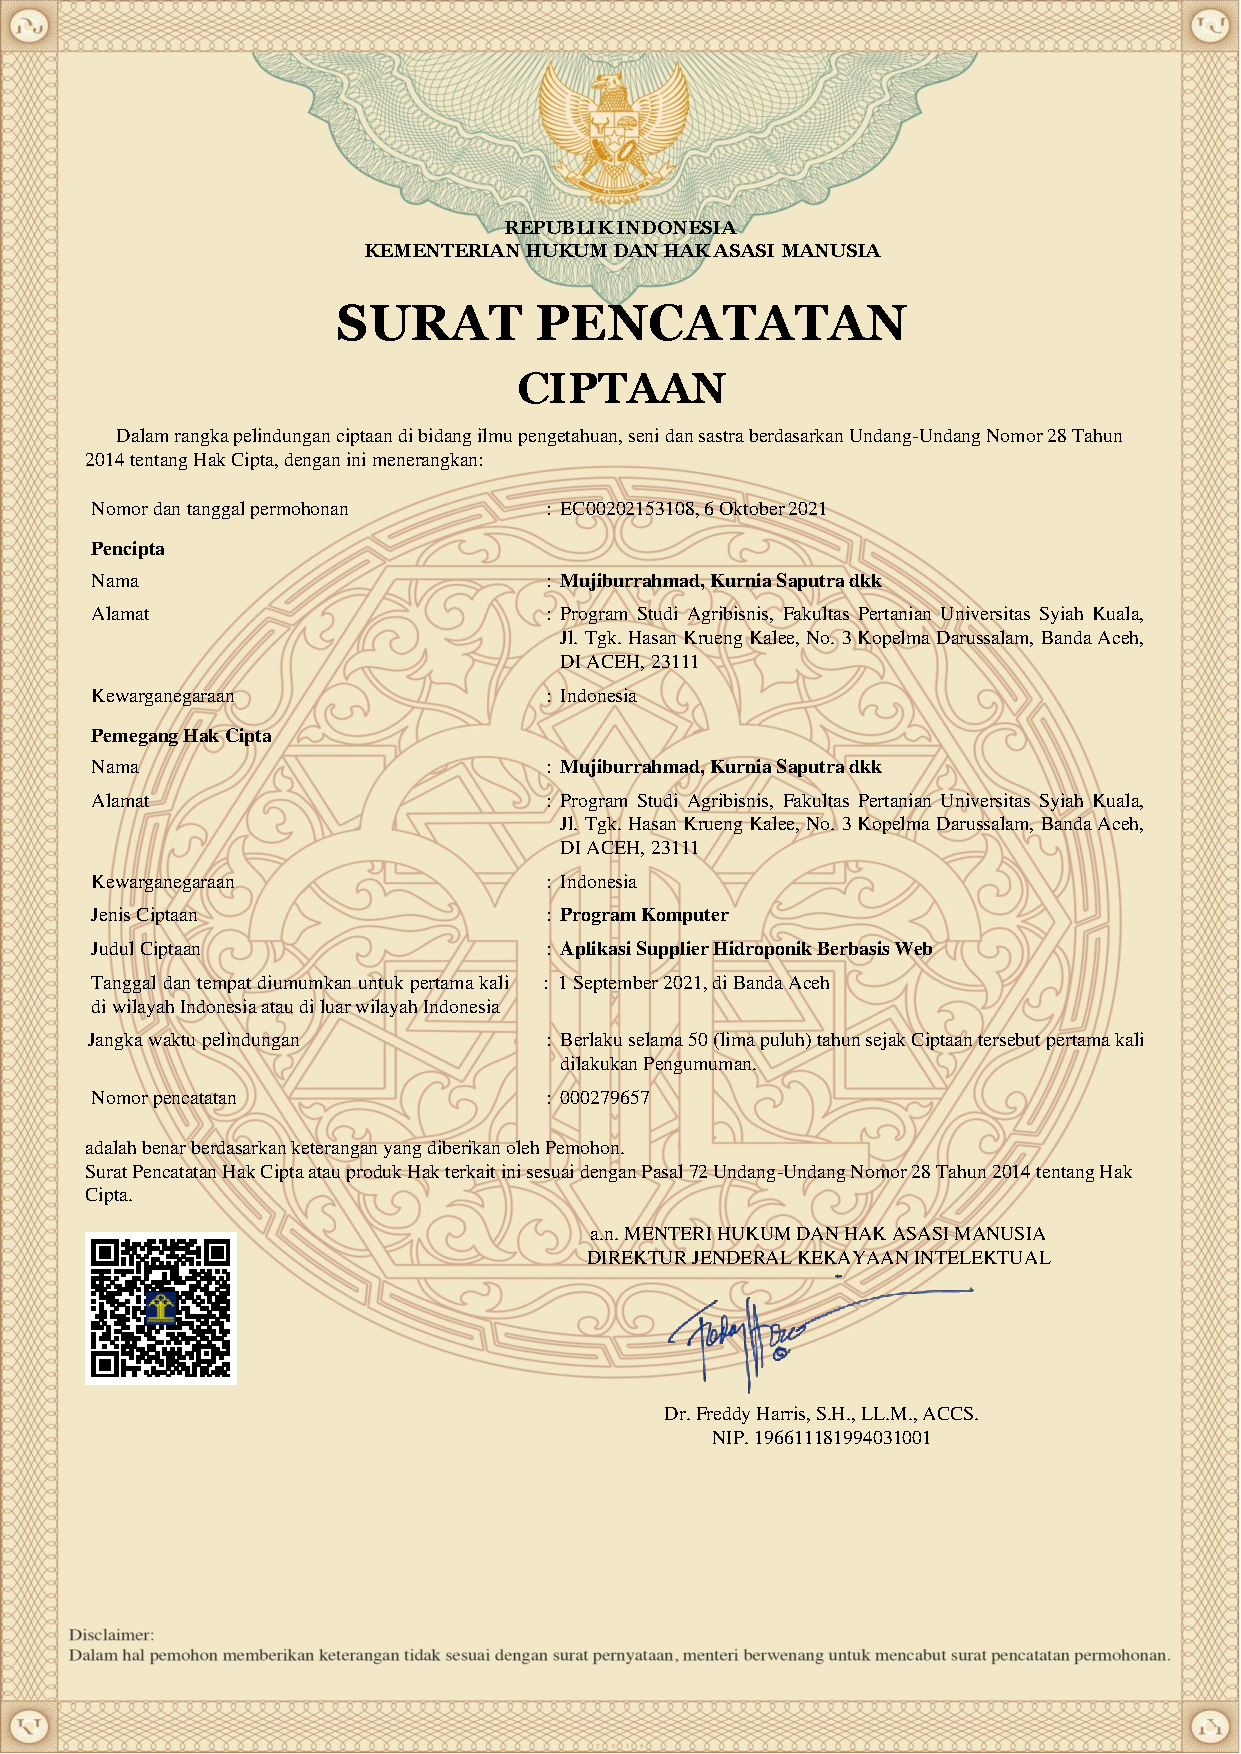
\includegraphics[width=13.3cm,height=18.3cm]{gambar/HKI.pdf}
    \end{figure}
\end{appendices}

\newpage

\fancyhf{} 
\fancyfoot[R]{\thepage}

\begin{appendices}{Lampiran 2. Foto Pengujian \textit{Usability}}
    \section*{Lampiran 2. Foto Pengujian \textit{Usability}}
    % \appendices{Lampiran 2. Foto Usability}
    \begin{figure}[H]
        % \begin{flushleft}
            \hspace*{0.8cm}
            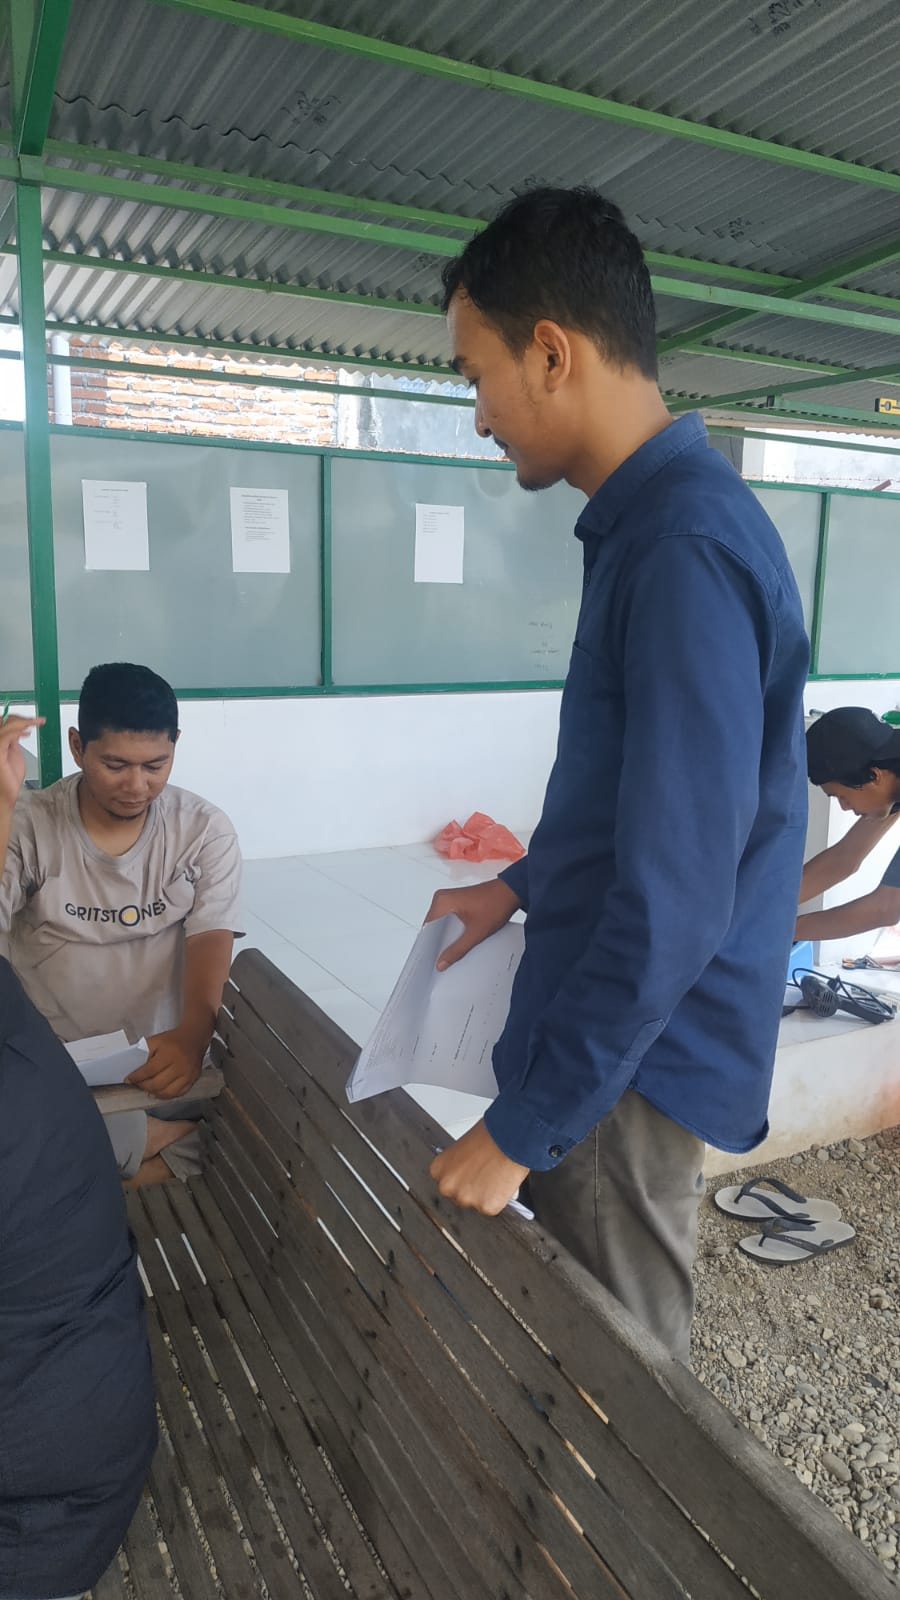
\includegraphics[width=5.5cm,height=9cm]{gambar/dokumentasi/foto1}
            \hspace*{0.3cm}
            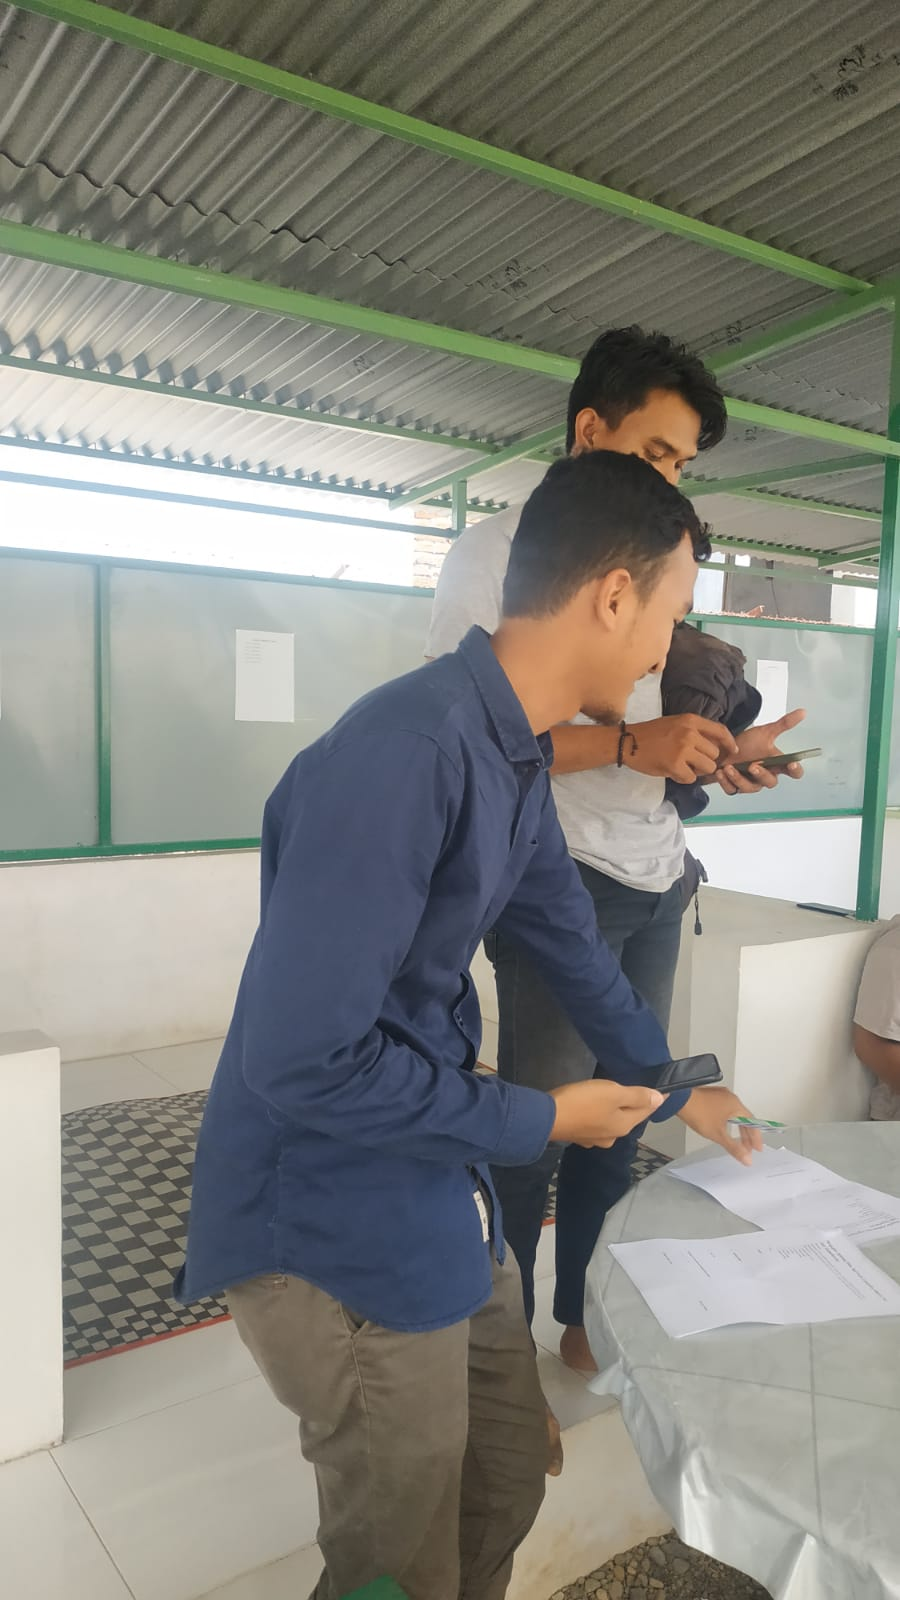
\includegraphics[width=5.5cm,height=9cm]{gambar/dokumentasi/foto2}
        % \end{flushleft}
    \end{figure}
    % \begin{figure}[H]
    %     \begin{flushright}
    %         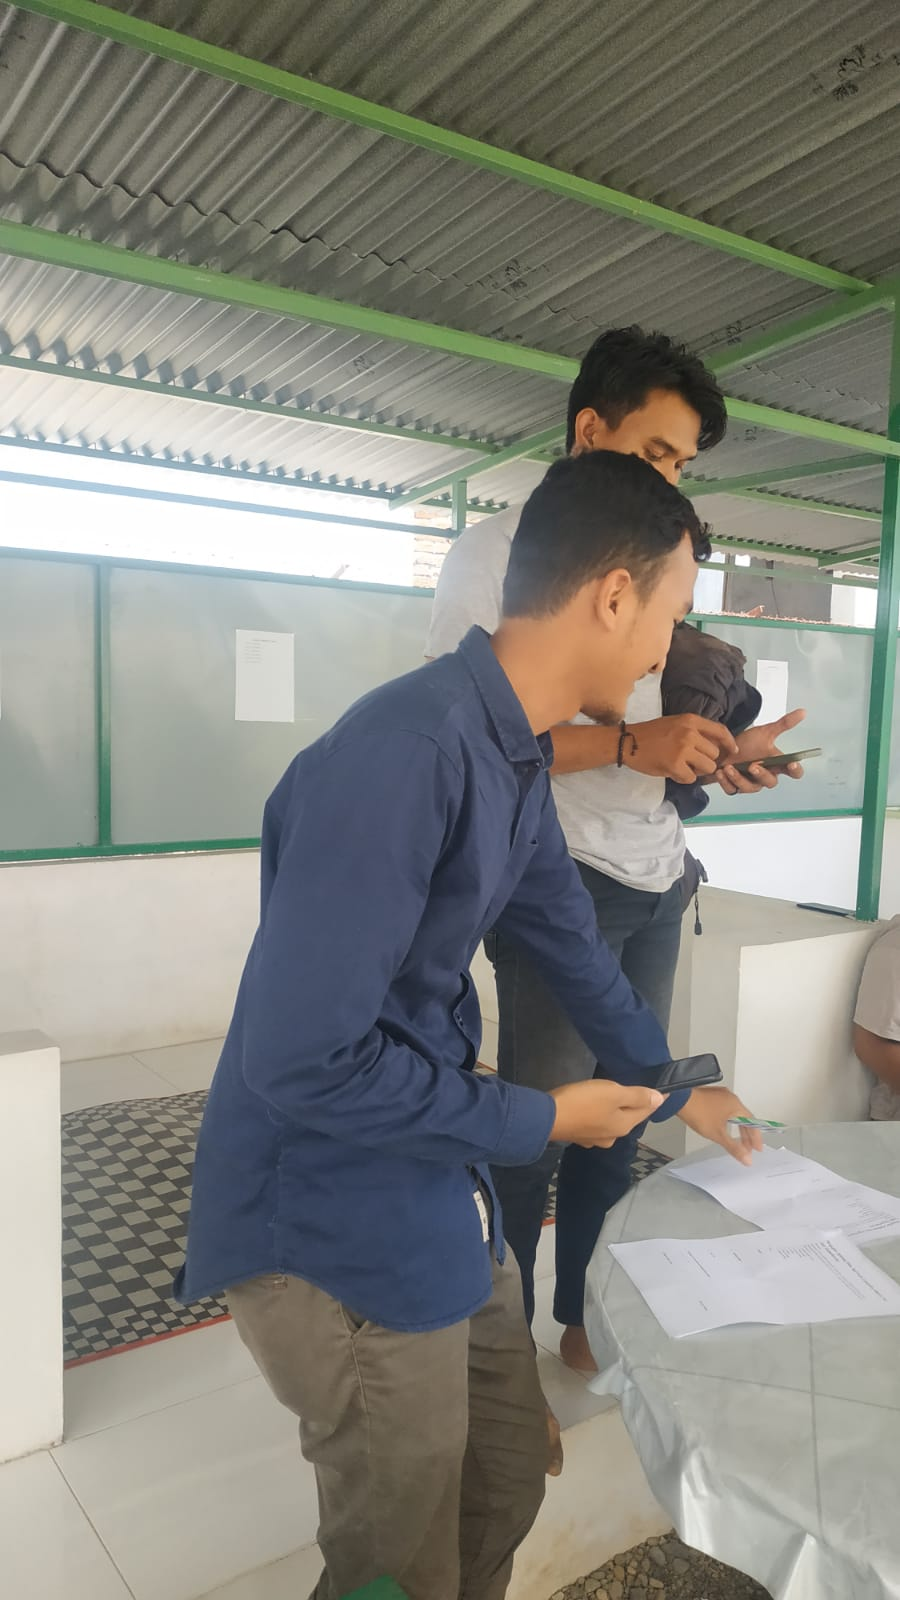
\includegraphics[width=6cm,height=9cm]{gambar/dokumentasi/foto2}
    %     \end{flushright}
        
    % \end{figure}
        
    % \begin{figure}[H]
    %     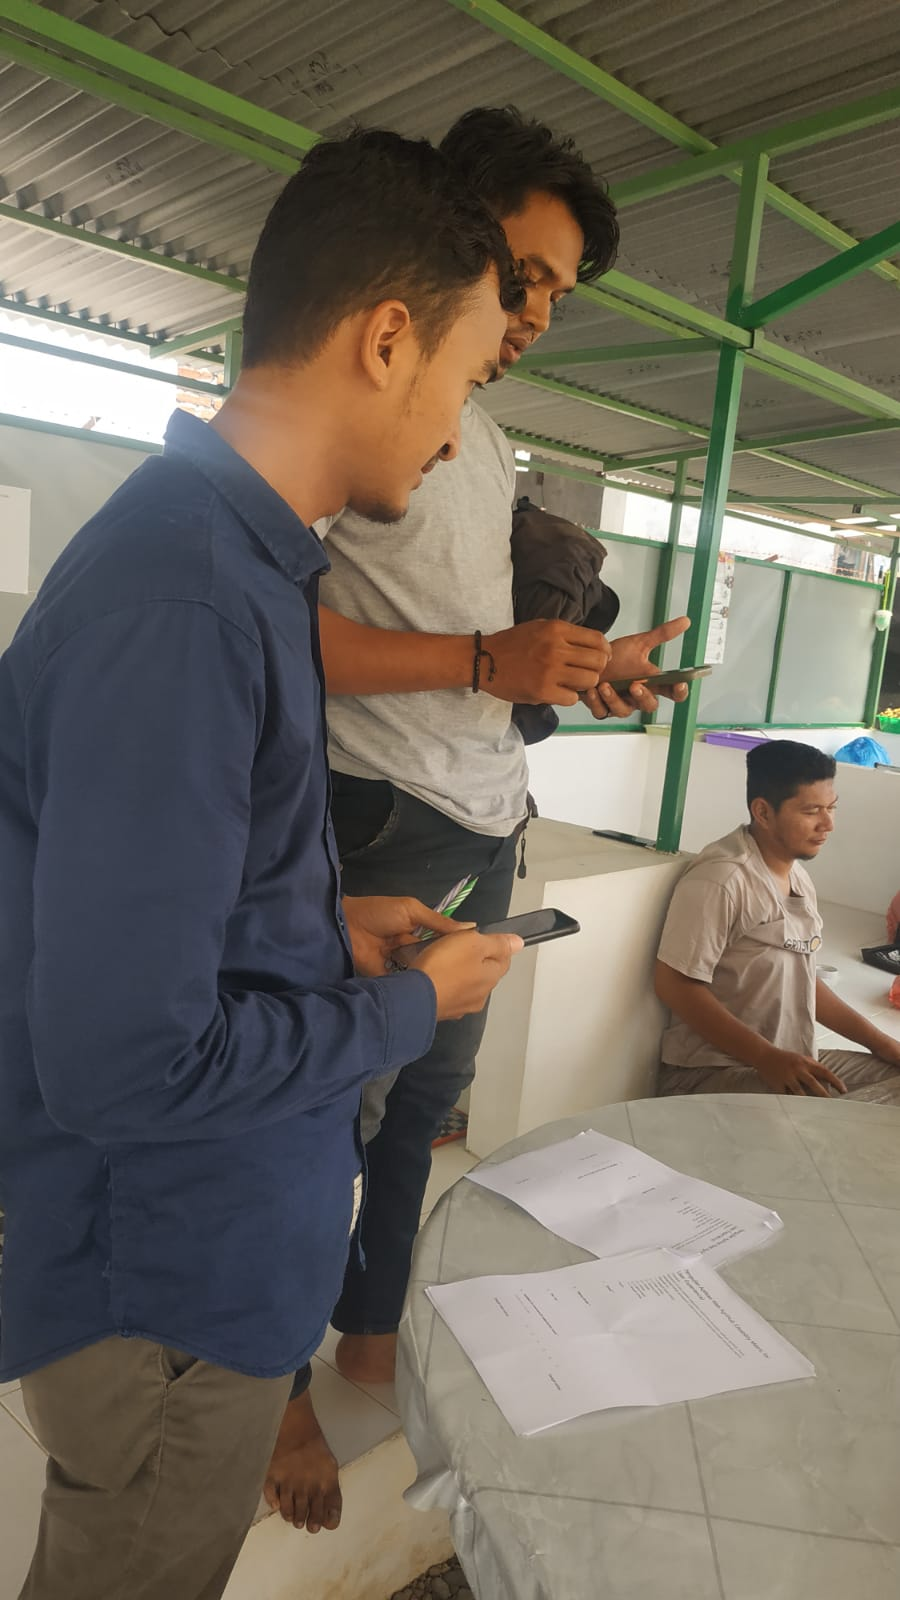
\includegraphics[width=8cm,height=12.5cm]{gambar/dokumentasi/foto3}
    % \end{figure}

    \begin{figure}[H]
        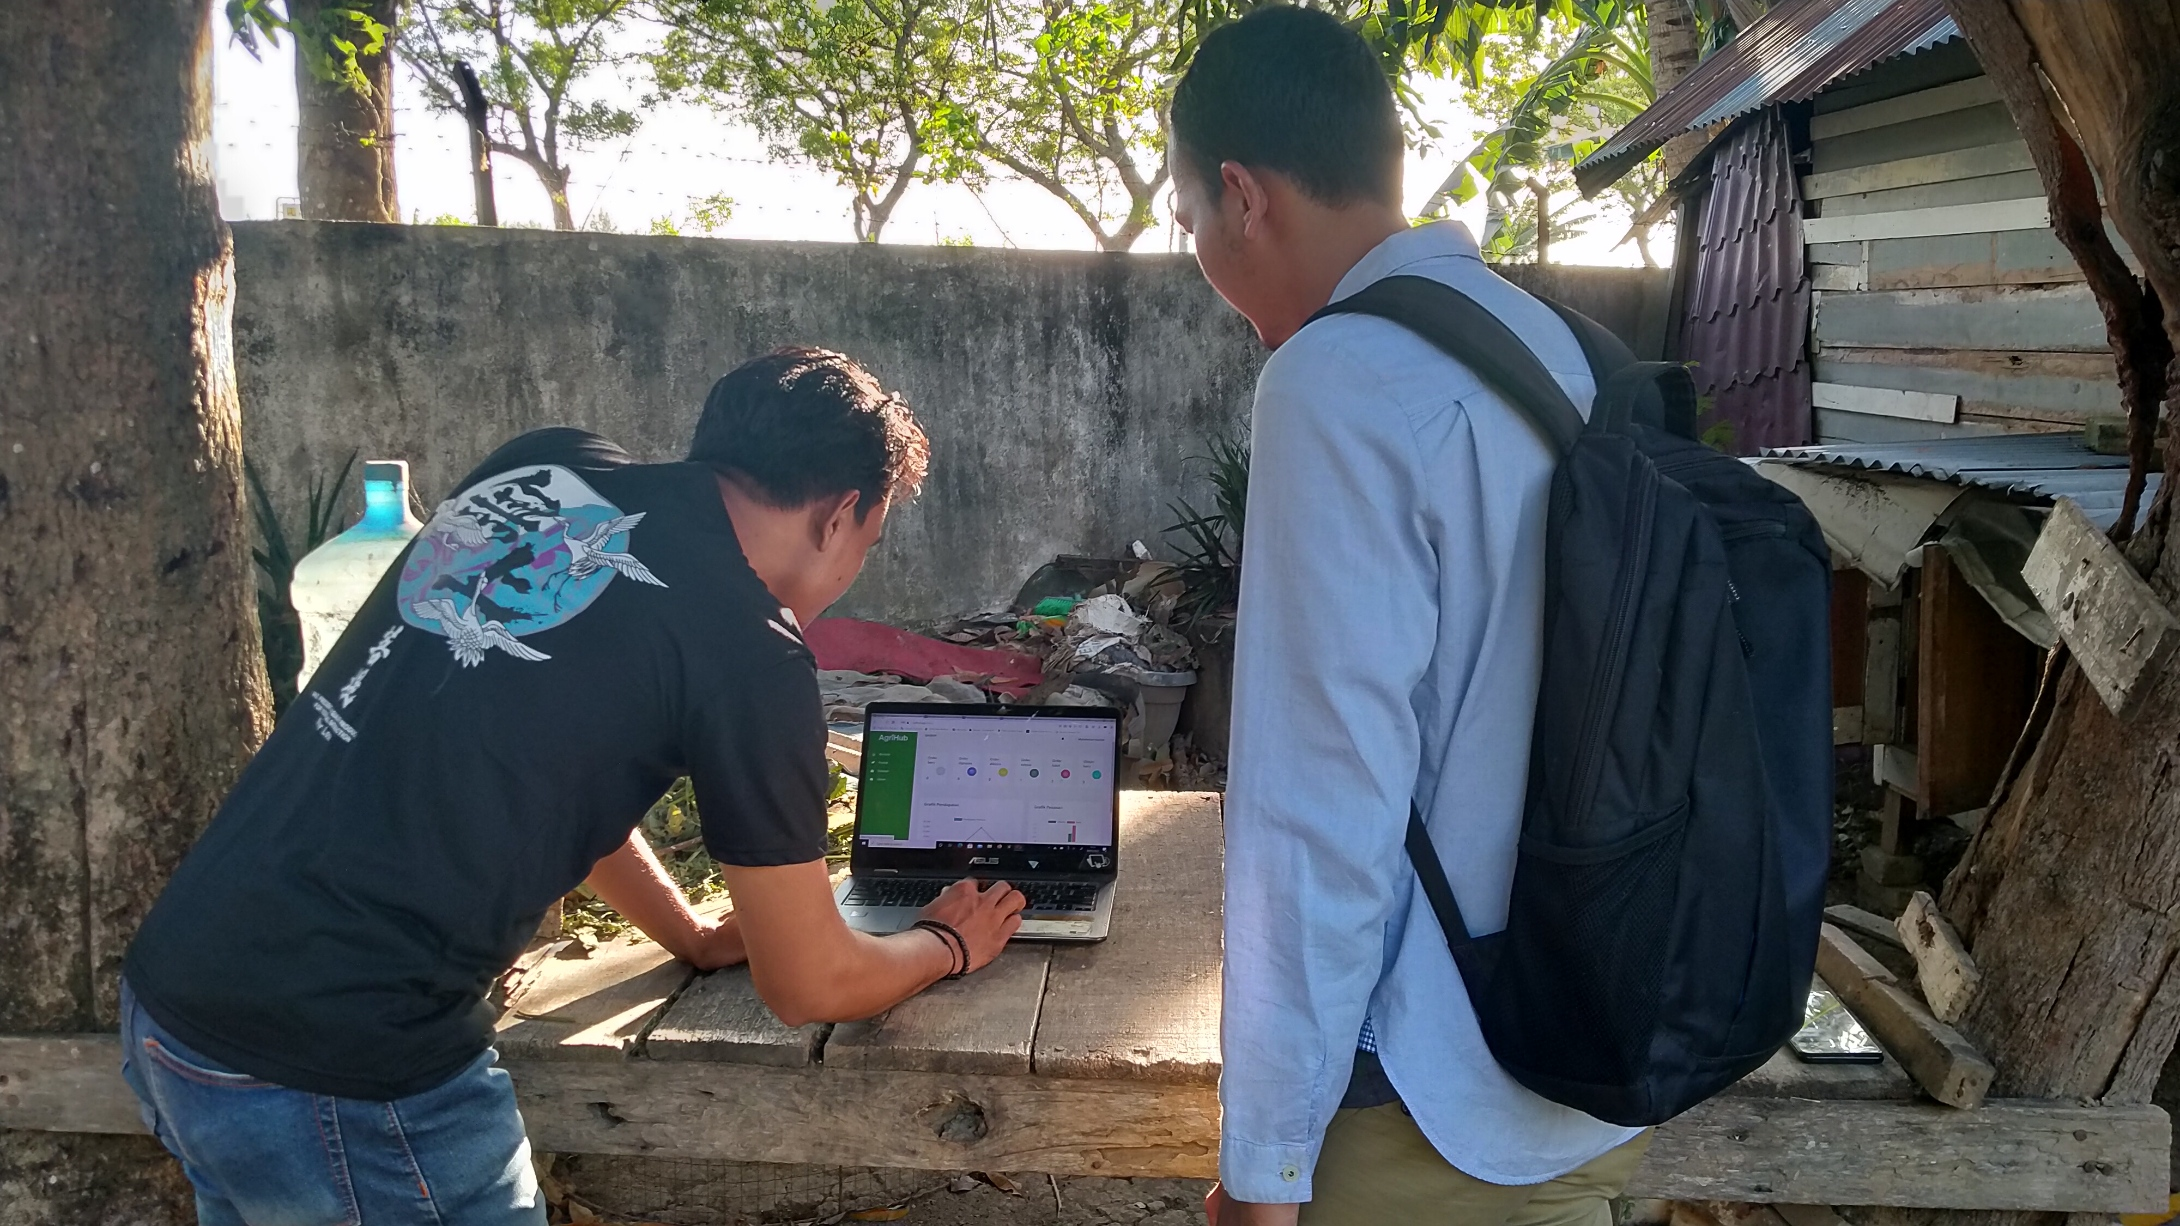
\includegraphics[width=6.5cm,height=4cm]{gambar/dokumentasi/foto7}
        \hspace*{0.2cm}
        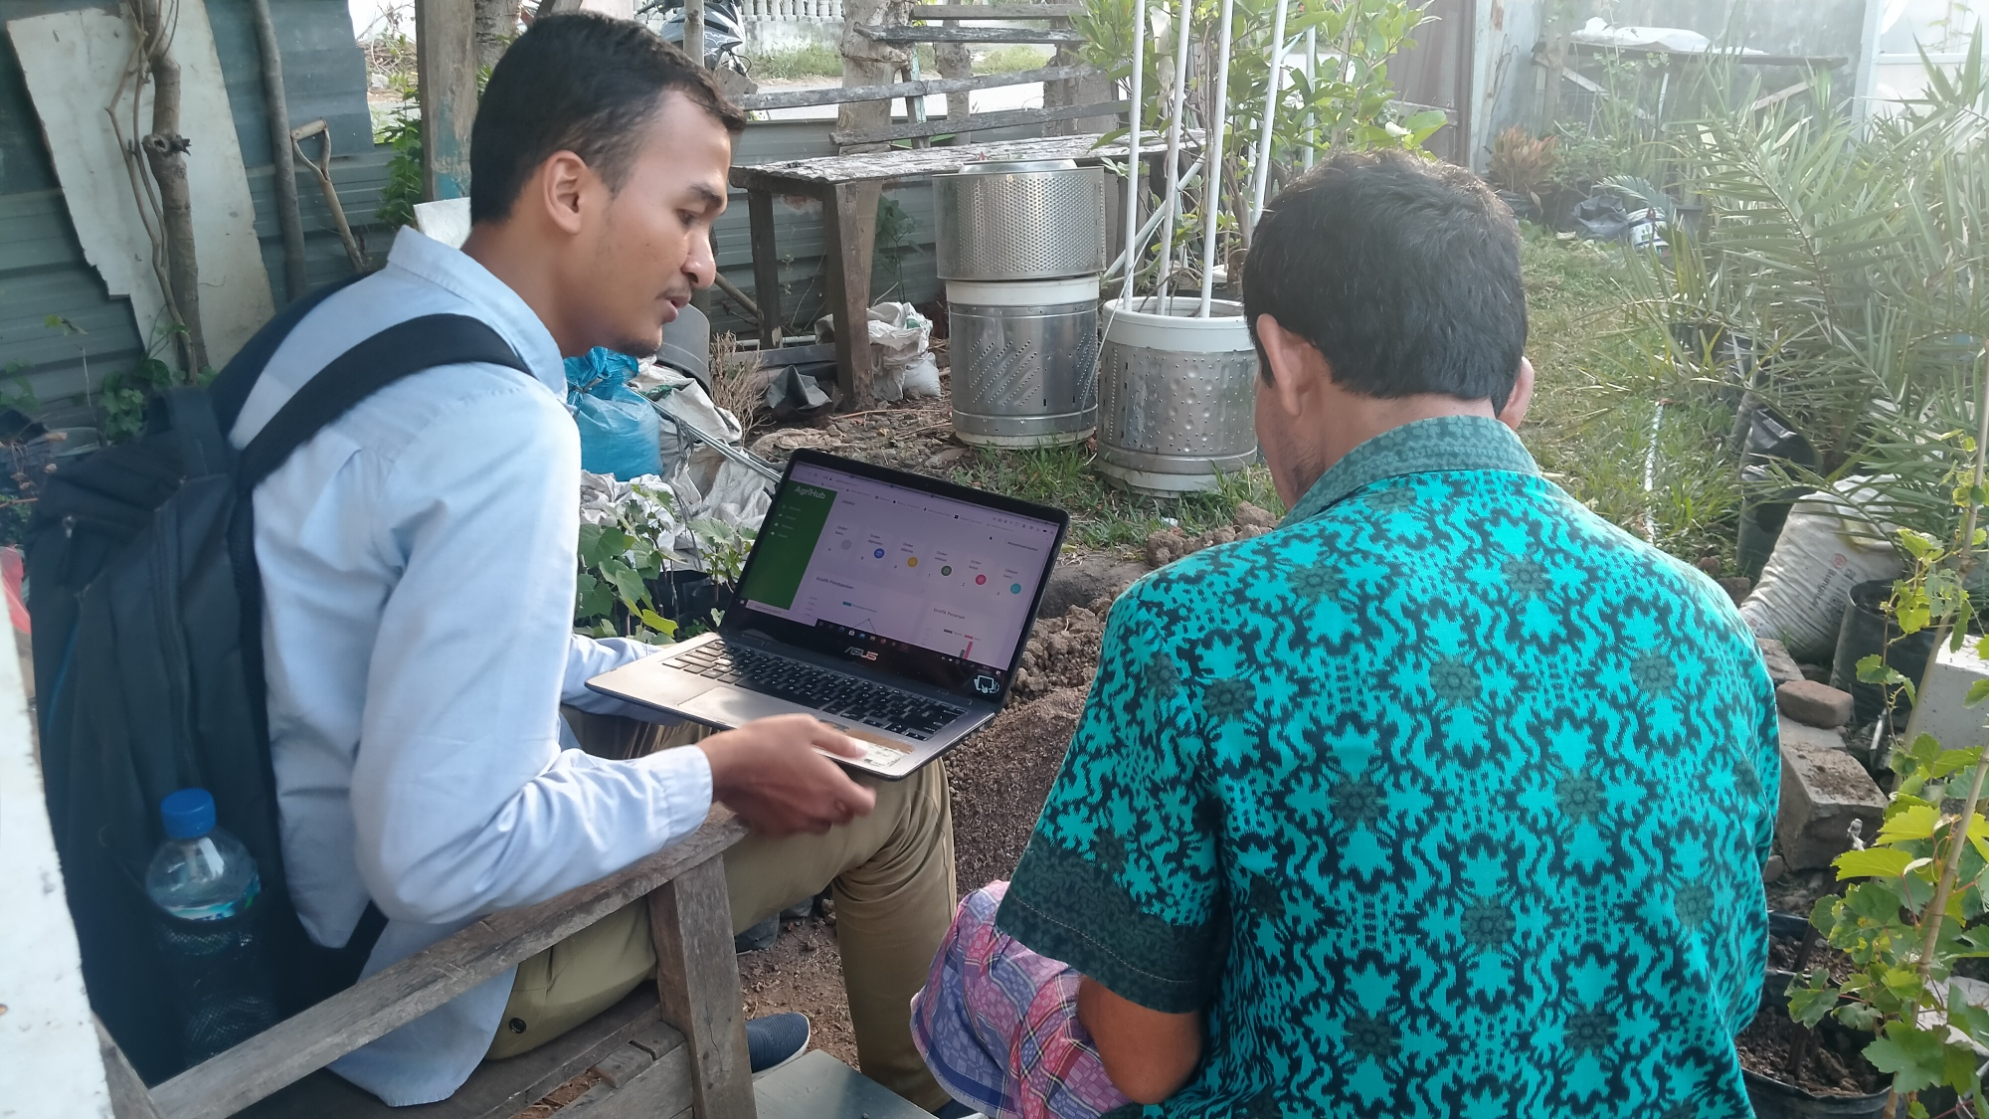
\includegraphics[width=6.5cm,height=4cm]{gambar/dokumentasi/foto8}
    \end{figure}
    \begin{figure}[H]
        \hspace*{1.5cm}
        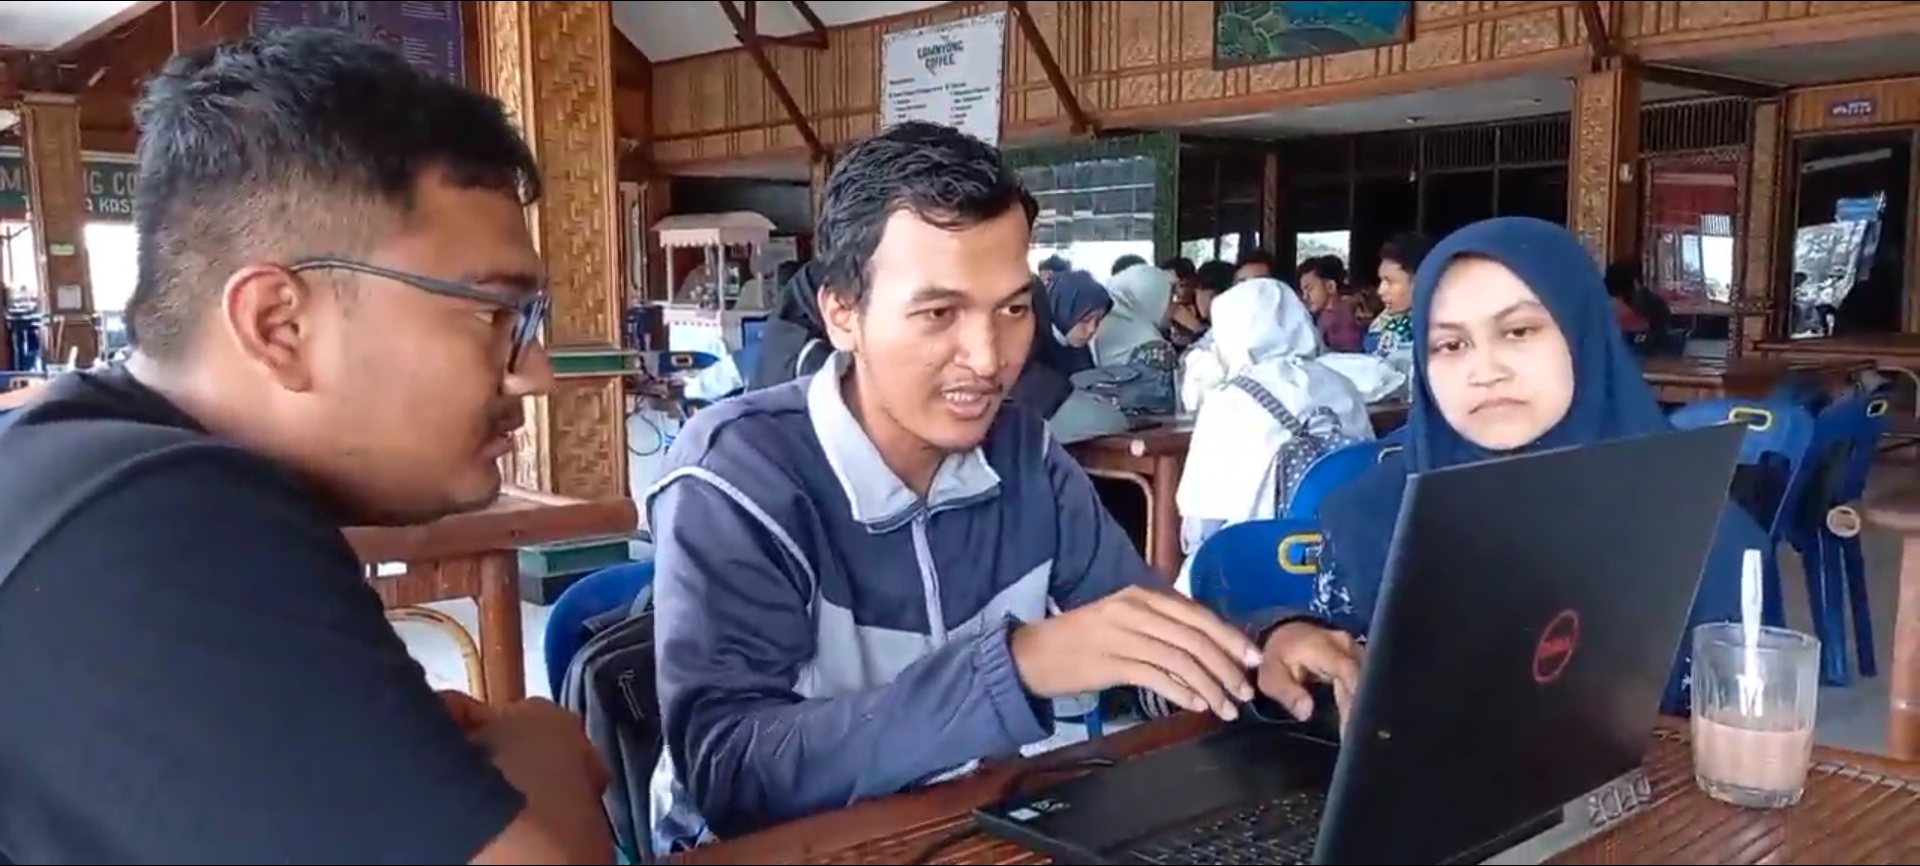
\includegraphics[width=10.5cm,height=5cm]{gambar/dokumentasi/doku testi}
    \end{figure}
        
        % 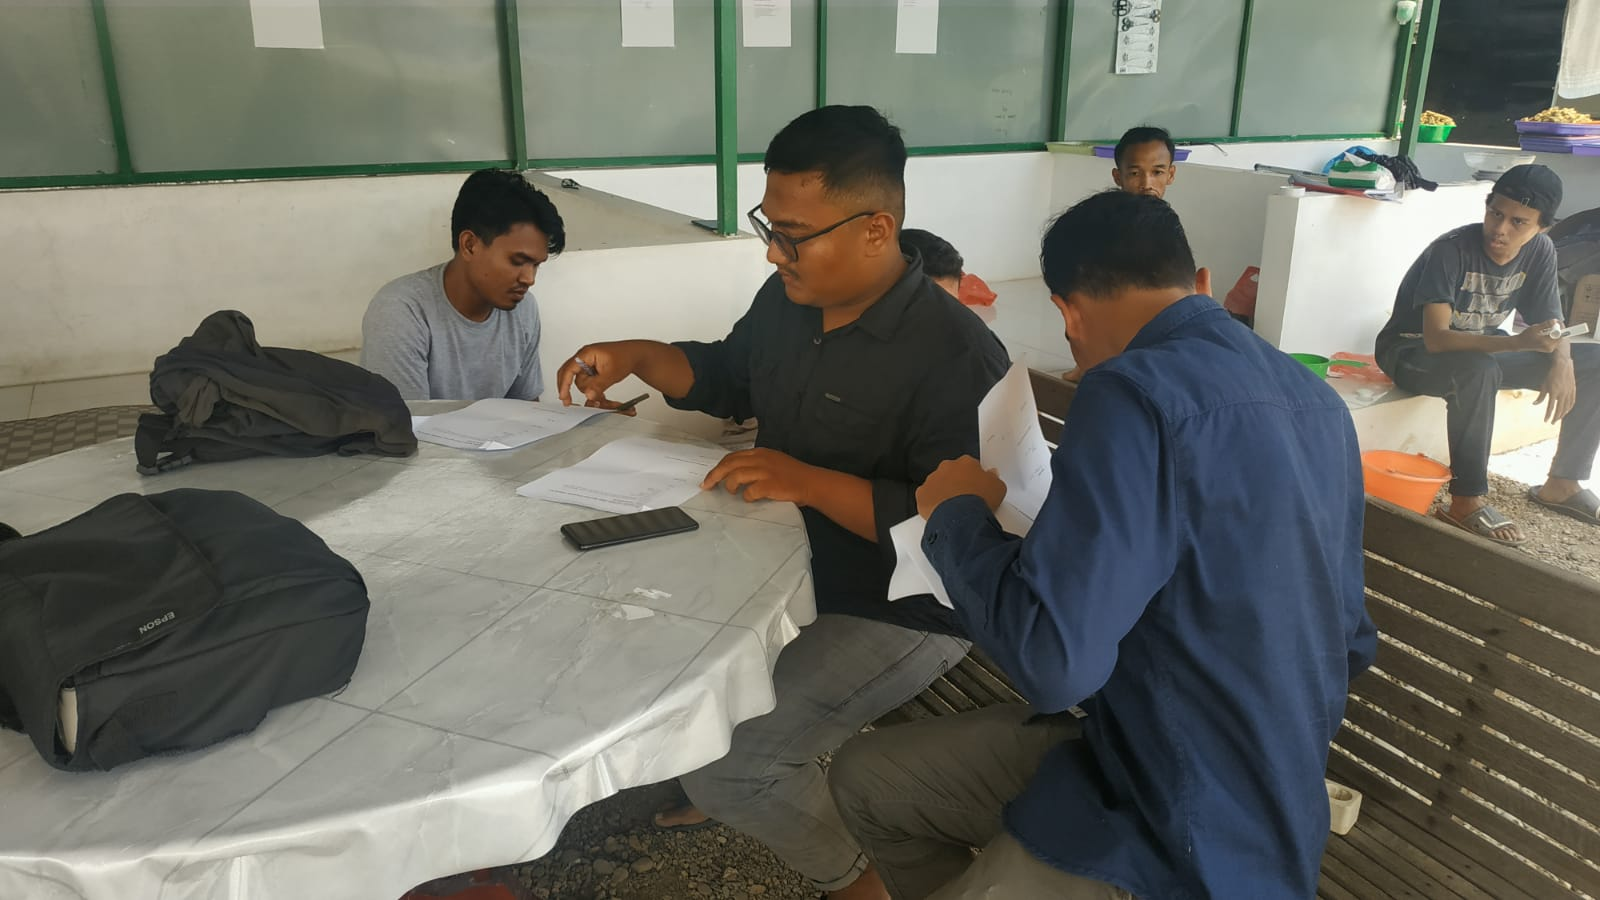
\includegraphics[width=12.5cm,height=8cm]{gambar/dokumentasi/foto5}
        
\end{appendices}

\newpage

\begin{appendices}{Lampiran 3. Foto Kegiatan Diskusi Bersama Klien}
    \section*{Lampiran 3. Foto Kegiatan Diskusi Bersama Klien}
    % \appendices{Lampiran 2. Foto Usability}
    \begin{figure}[H]
        % \begin{flushleft}
            % \hspace*{0.2cm}
            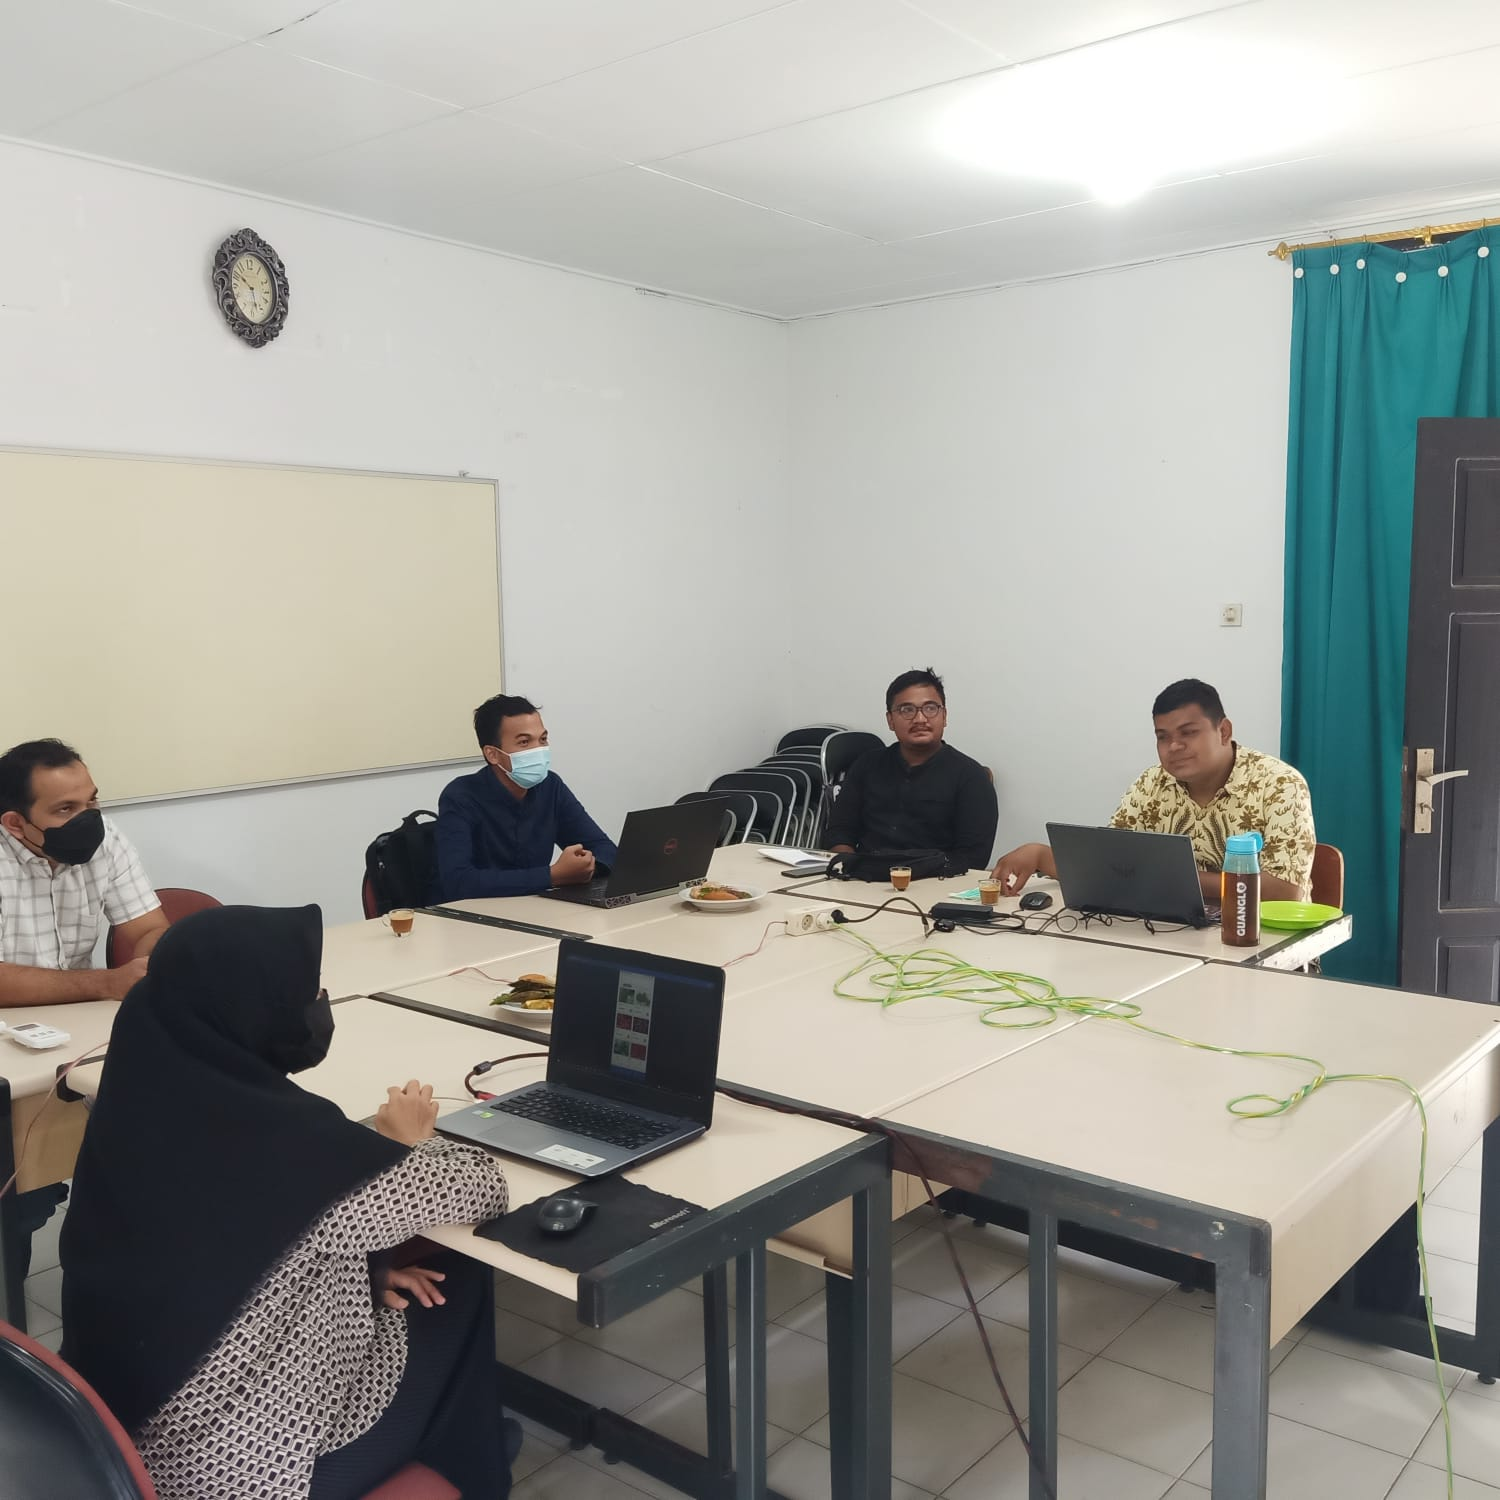
\includegraphics[width=6.5cm,height=6.5cm]{gambar/dokumentasi/diskusi1}
            \hspace*{0.3cm}
            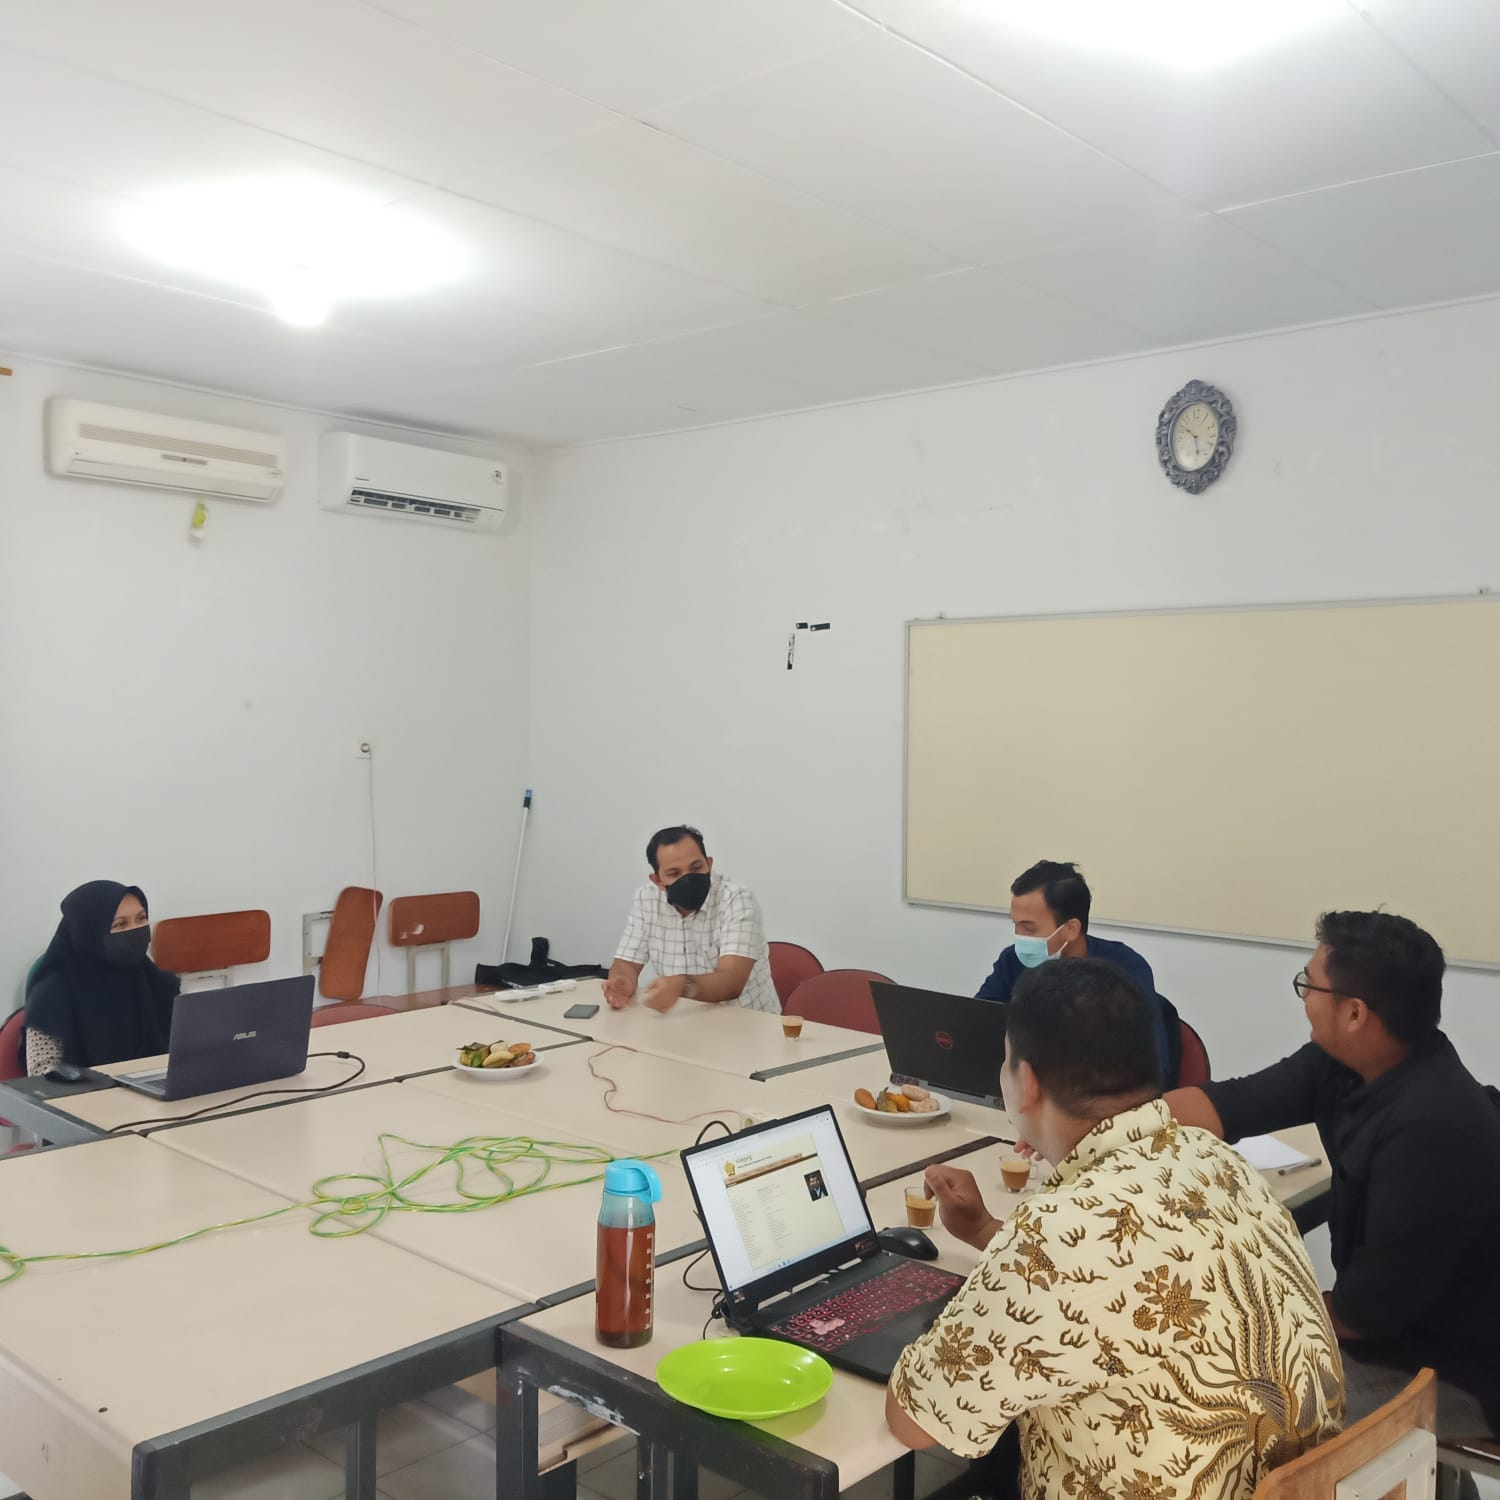
\includegraphics[width=6.5cm,height=6.5cm]{gambar/dokumentasi/diskusi2}
        % \end{flushleft}
    \end{figure}
\end{appendices}

% \begin{appendices}{Lampiran 2}
%     Lampiran 2. Foto Usability Testing
%     \begin{figure}
%         \flushleft
%         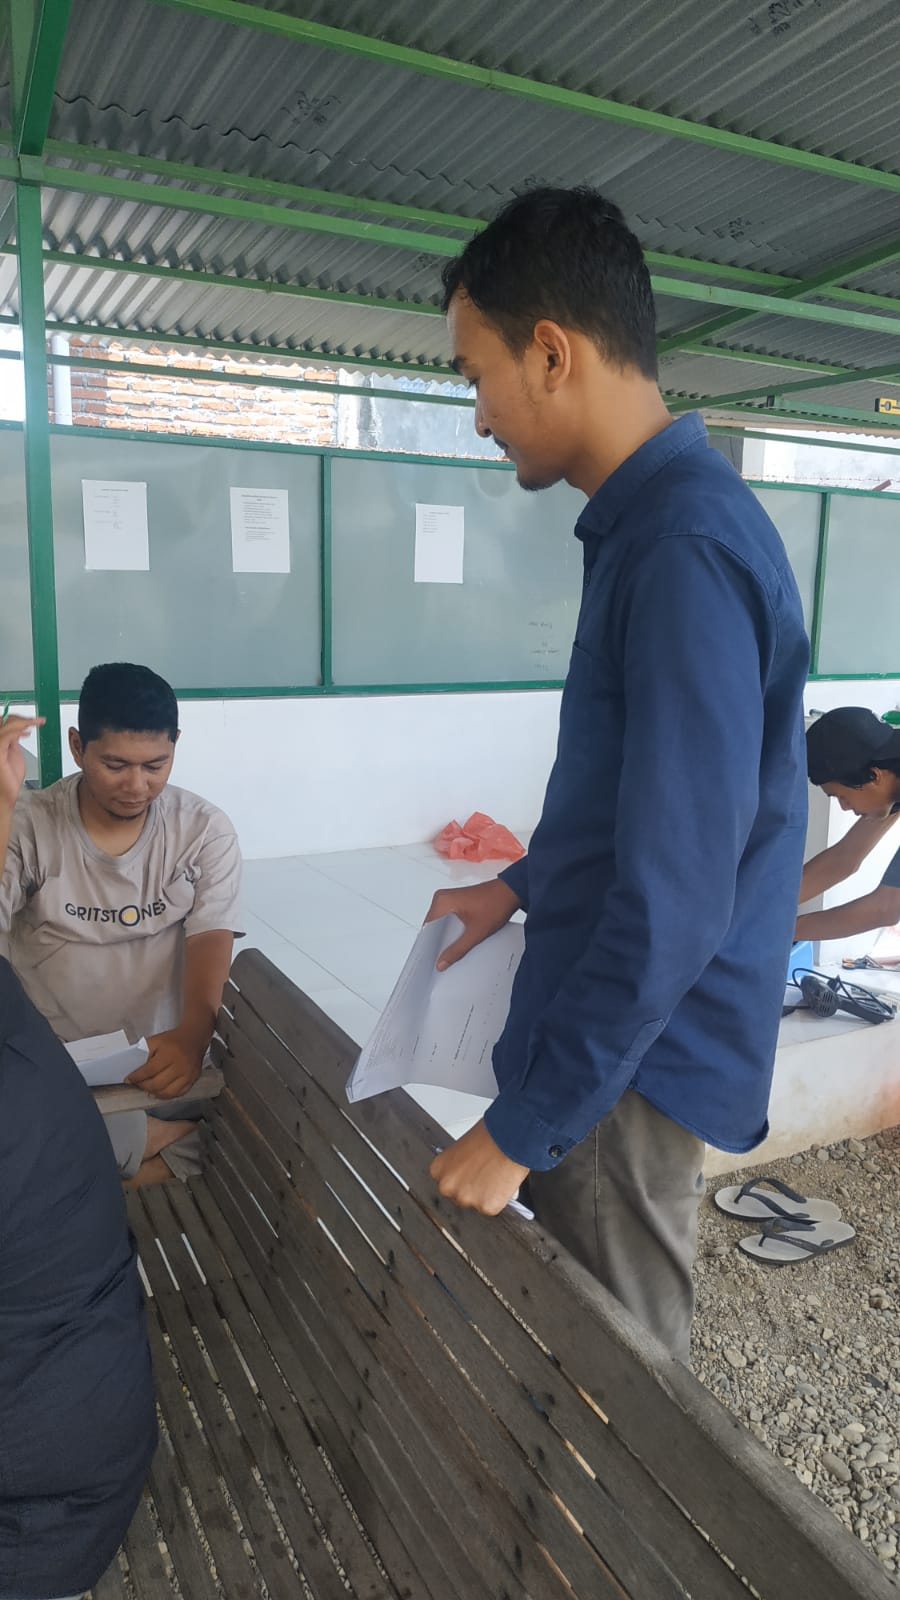
\includegraphics[width=5cm,height=9.5cm]{gambar/dokumentasi/foto1}
%         \flushright
%         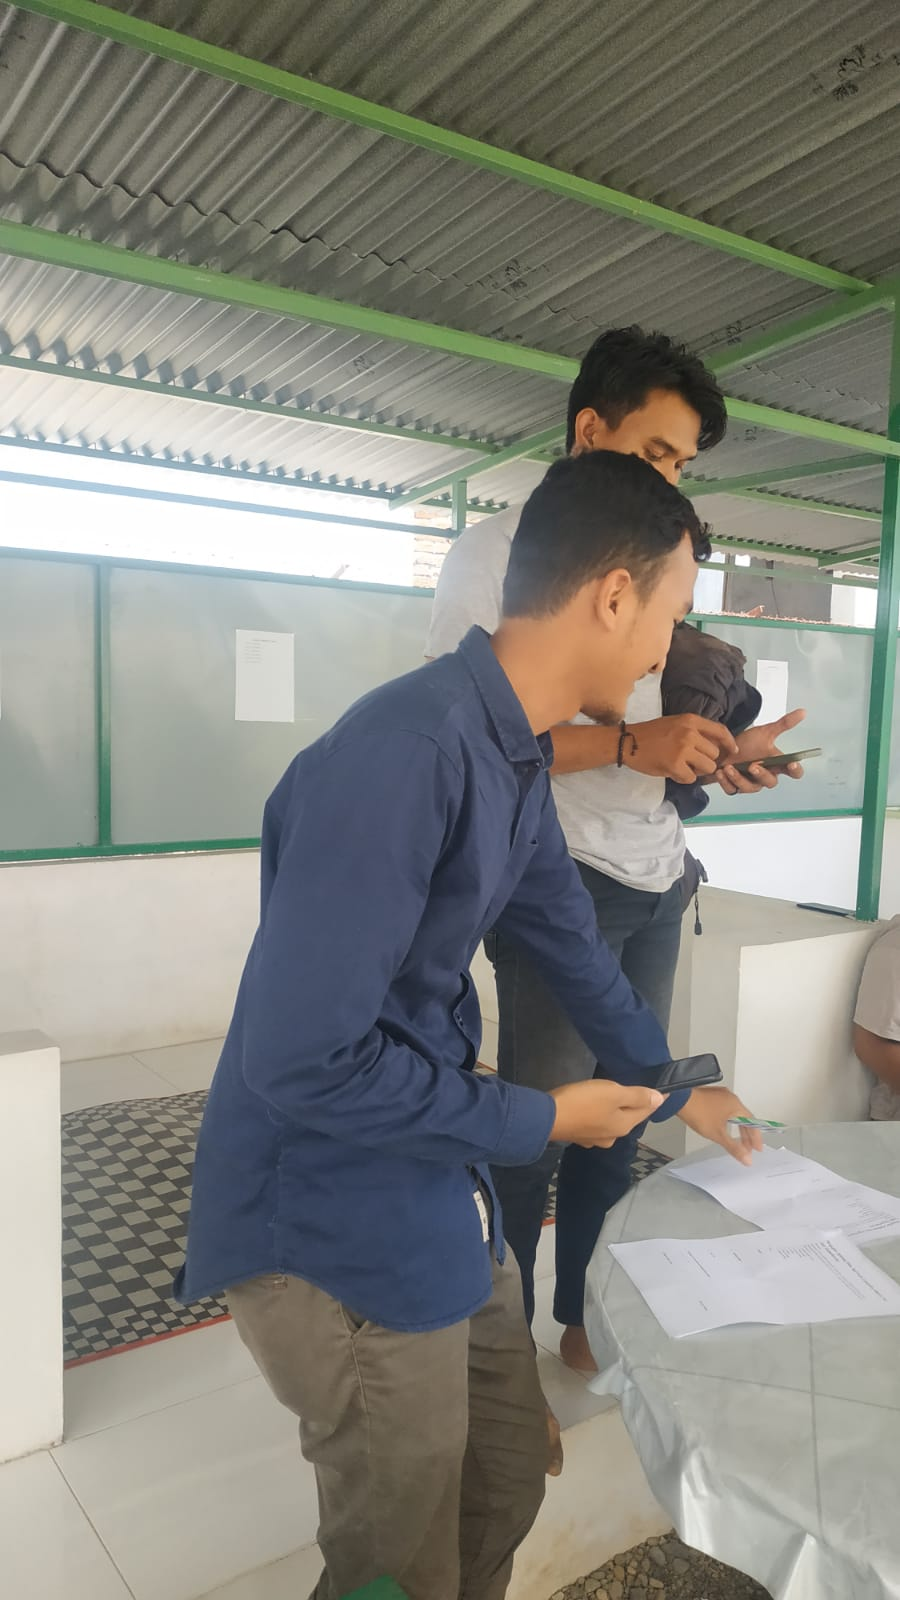
\includegraphics[width=5cm,height=9.5cm]{gambar/dokumentasi/foto2}
%     \end{figure}
%     \begin{figure}
%         
%         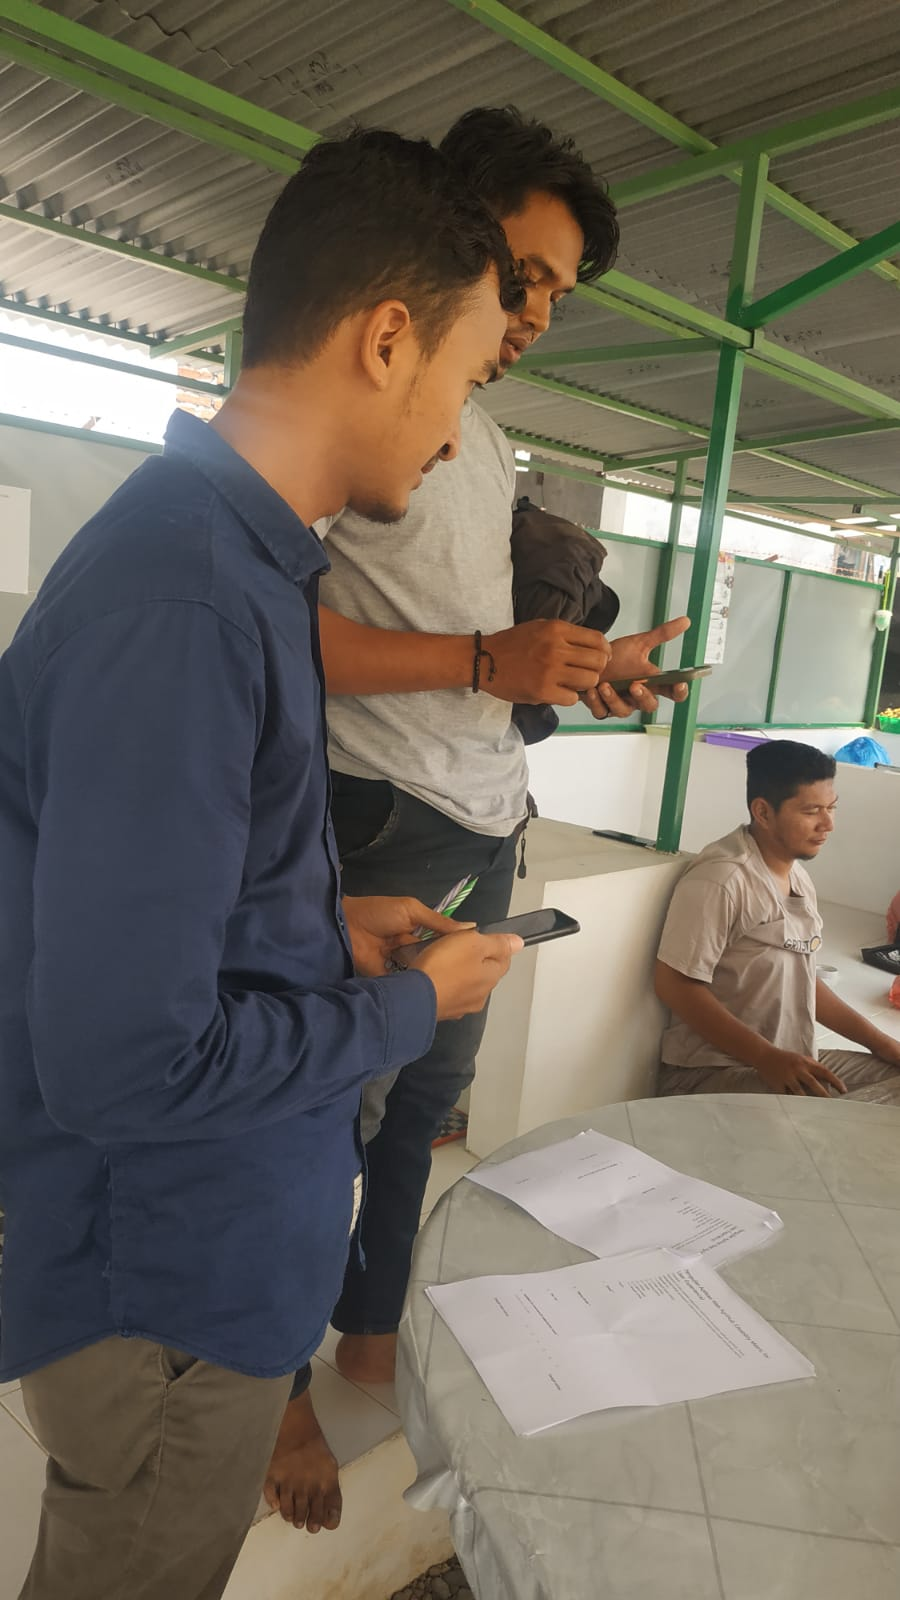
\includegraphics[width=8cm,height=12.5cm]{gambar/dokumentasi/foto3}
%     \end{figure}
%     \begin{figure}
%         \centering
%         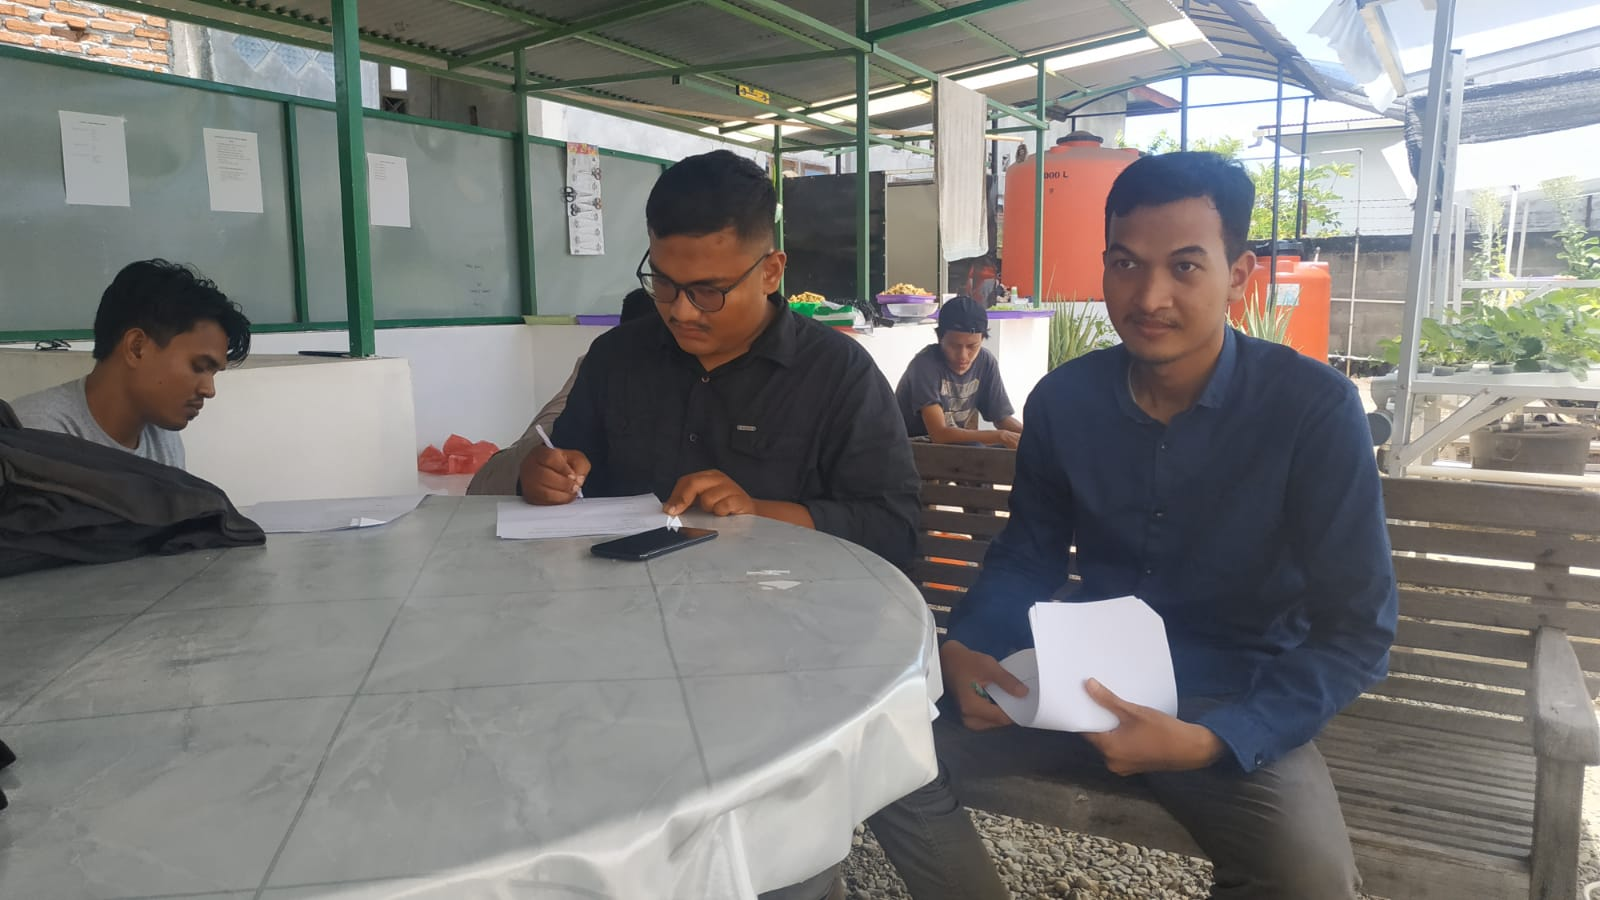
\includegraphics[width=12.5cm,height=8cm]{gambar/dokumentasi/foto4}
%     \end{figure}
%     \begin{figure}
%         \centering
%         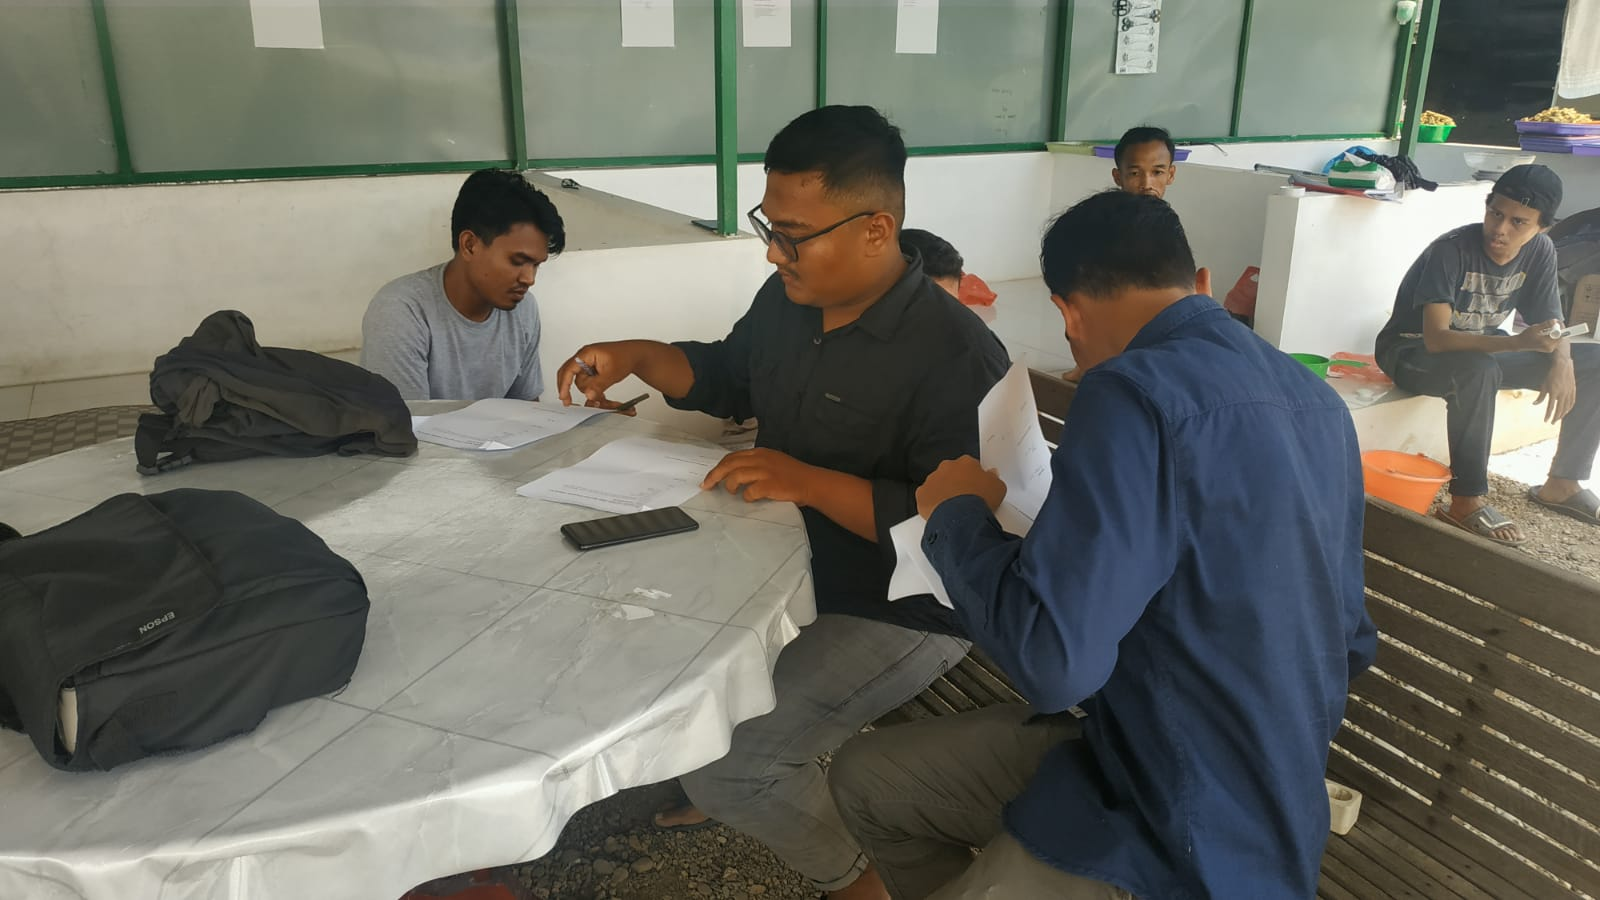
\includegraphics[width=12.5cm,height=8cm]{gambar/dokumentasi/foto5}
%     \end{figure}
%     \begin{figure}
%         \centering
%         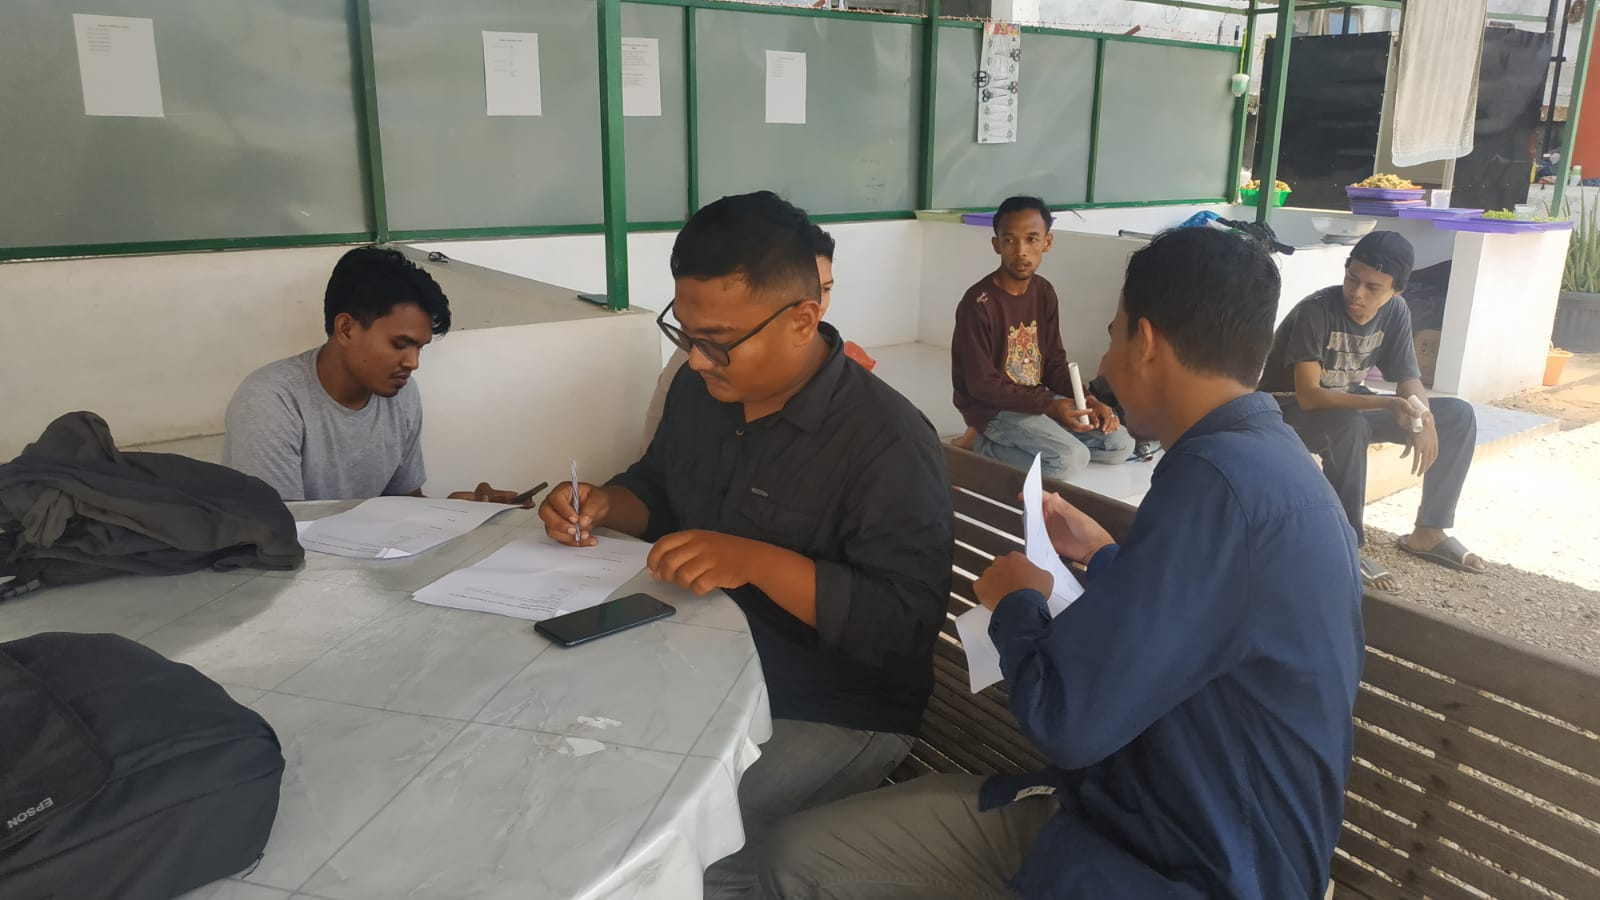
\includegraphics[width=12.5cm,height=8cm]{gambar/dokumentasi/foto6}
%     \end{figure}
% \end{appendices}

\newpage
\begin{center}
    \large{\textbf{BIODATA}}
\end{center}

\vspace*{0.5cm}

\begin{enumerate}
    \item Nama :
    \item Tempat, tanggal lahir :
    \item Alamat :
    \item Nama Ayah :
    \item Pekerjaan Ayah :
    \item Nama Ibu :
    \item Pekerjaan Ibu :
    \item Alamat Orang Tua :
    \item Riwayat Pendidikan :
        \hspace*{1cm}
        \begin{table}[h!]
            \begin{tabular}{|l|l|l|l|l|} % Membuat garis vertikal
            \hline % Membuat garis horizontal pertama
            Jenjang & Nama Sekolah & Bidang Studi & Tempat & Tahun Ijazah\\
            \hline % Membuat garis horizontal kedua
            SD   & & & & \\
            \hline
            SLTP   & & & & \\
            \hline
            SLTA   & & & & \\
            \hline
            Diploma  & & & & \\
            \hline % Membuat garis horizontal ketiga
            \end{tabular}
        \end{table}
    \item Karya Tulis
        \hspace*{1cm}
        \begin{table}[h!]
            \begin{tabular}{|c|l|l|l|} % Membuat garis vertikal
            \hline % Membuat garis horizontal pertama
            No. & Judul & Tahun & Penerbit\\
            \hline % Membuat garis horizontal kedua
            1   & & & \\
            \hline
            2   & & & \\
            \hline % Membuat garis horizontal ketiga
            \end{tabular}
        \end{table}
\end{enumerate}

\begin{tabular}{p{7.5cm}c}
	&Banda Aceh, 24 Agustus 2022\\
	&\\
	&\\
	&\\
	&\underline{Muhammad Kautsar}\\
	&16080107010020
\end{tabular}

\newpage
\begin{center}
    \large{\textbf{PERNYATAAN PERSETUJUAN PUBLIKASI DAN EMBARGO KARYA TULIS CIVITAS AKADEMIKA UNSYIAH}}
\end{center}

\vspace*{0.5cm}
Saya yang bertanda tangan di bawah ini :
\newline
\hspace*{2cm}
\begin{tabular}{l}
	Nama :\\
	NPM/NIP :\\
	Judul :\\
	Fakultas :\\
	Jurusan :\\
	Program Studi :
\end{tabular}

\vspace*{0.5cm}
menyetujui:
\newline
( ) untuk mengunggah softcopy Tugas Akhir/Tesis saya diatas secara penuh atau full-text
di Repository Perpustakaan Unsyiah dan diakses atau terbaca lewat mesin pencari
internet secara publik
\newline
( ) untuk mengunggah softcopy Tugas Akhir/Tesis kami diatas secara parsial atau hanya bagian Tertentu (misalnya Cover, Lembar Pengesahan, Abstrak, Daftar Isi, Pendahuluan dan Kesimpulan) ke Repository Perpustakaan Unsyiah dan diakses atau terbaca lewat mesin pencari internet secara publik
\newline
( ) untuk tidak membolehkan sama sekali bagian Tugas Akhir/Tesis diakses online sampai dengan ............... (tulis tanggal, bulan, tahun; atau selamanya/tidak terhingga) dengan alasan: ...........................................................................................................................................
...........................................................................................................................................
dan setuju memberikan atau mengunggah softcopy Tugas Akhir/Tesis kepada Perpustakaan Unsyiah secara penuh dalam bentuk PDF untuk disimpan secara private ke dalam Repository yang tidak bisa dijangkau oleh mesin pencari (mis. Google).
\newline
Demikian pernyataan ini dibuat untuk dipergunakan sebagaimana mestinya.

\vspace*{0.5cm}

\begin{tabular}{p{7.5cm}c}
	&Banda Aceh, 24 Agustus 2022\\
	&\\
	&\\
	&\\
	&Muhammad Kautsar\\
	&16080107010020
\end{tabular}